\documentclass[margin,line,11pt]{article}
\usepackage[utf8]{inputenc}
\usepackage{amsmath}
\usepackage{graphicx}

\oddsidemargin -.5in
\evensidemargin -.5in
\topmargin -.75in
\textwidth=7.5in
\textheight=9.5in
\itemsep=0in
\parsep=0in

\title{Implementing compartmental models for infectious disease dynamics - Supplementary Material}
\author{Pulliam, JRC {\em et al}.}
\date{2020 (CC-BY)}

\begin{document}
%\begin{spacing}{1.5}

\maketitle


\section{The SIR Model World}

All implementations of the SIR model world, as shown here and in Figure 1A, have certain features in common. 
As described in the main text, this includes having three compartments (susceptible, infected, and removed) as well as two processes (transmission and removal). 
By default, implementations of this model world also assume that  populations are well mixed (i.e., each individual is equally likely to contact any other individual in the population) and that the rate at which a susceptible makes effective contacts remains constant. The latter can have subtle implications for interpretation; if ``removal'' includes death, then this assumption implies replacing the contacts that would have been made with dead individuals by additional contact with individuals that remain in the population.

\begin{figure}[h]
    \centering
    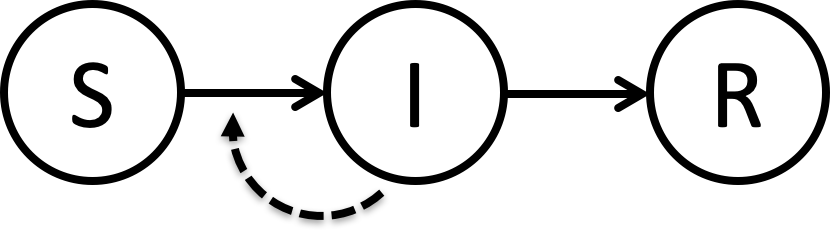
\includegraphics{SIR.png}
    \caption{The SIR model world.}
    \label{fig:my_label}
\end{figure}

\section{The SIR Model Family}

In the main text, we introduce the SIR model world and the idea that it can be implemented using many different model specifications. 
Here, we discuss six different models within the SIR model family. 
These implementations are not intended to be exhaustive, but rather to demonstrate common options representing various positions in the model taxonomy. 
Modifications to the model world, e.g. considering an exposed class with an SEIR model, could be accommodated with corresponding modifications to the implementations resulting in a new family of models; this can be done for any compartmental model world.
In addition, code is available for each of these six implementations, and we encourage readers to make use of the code snippets as a starting point for building more complex models.

\subsection{Model 1: Ordinary differential equations}

The most common implementation of the SIR model world is the deterministic ordinary differential equation (ODE) SIR model. 
In this implementation, time is represented as a continuous quantity; the rate at which new infections are being created is represented as $\beta S I / N$, and the rate at which individuals are leaving the infected class is represented as $\gamma I$, where $\beta$ is the {\em per capita} rate at which potentially infectious (``effecive'') contacts occur, $\gamma$ is the rate of recovery events (equivalent to the reciprocal of the average duration of infectiousness), and $N=S+I+R$ is the total population size. 
The population is assumed to be sufficiently large that the system exhibits the average behavior. 
This assumption allows individuals to be represented as continuous quantities (averages or densities) and implies that a given set of initial conditions and values for the model parameters ($\beta$ and $\gamma$, or $R_0$, the threshold quantity) will always produce the same outcome. 
In this implementation, the model equations are:

\begin{eqnarray*}
\frac{dS}{d\tau} &=& -\frac{\beta S I}{N}\\
\frac{dI}{d\tau} &=& \frac{\beta S I}{N} - \gamma I \\
\frac{dR}{d\tau} &=& \gamma I
\end{eqnarray*}

\noindent Since $R_0 = \beta / \gamma$, as discussed in the main text, the number of parameters in the model can be reduced by rescaling time such that $t = \tau * \gamma$. 
This is equivalent to specifying time in units of the infectious period. The equations can thus be rewritten as:

\begin{eqnarray}
\frac{dS}{d\tau} &=& -\frac{R_0 S I}{N}\label{eqn:1} \\
\frac{dI}{d\tau} &=& \frac{R_0 S I}{N} - I\label{eqn:2}
\end{eqnarray}

\noindent Note that the model can specified by stating only two of the rate equations because the total population size $N$ is constant (e.g. the rate equation for $R$ need not be specified when those of $S$ and $I$ are specified since $R=N-S-I$). In addition, the model could be rescaled by the population size to further reduce the dimensionality; however, we have not done this here for the sake of consistency of representation with other model implementations.

% add psuedocode?

\subsection{Model 2: The Gillespie algorithm}

The Gillespie algorithm [REF: Gillespie, Feller et al] provides a direct stochastic analogue to the ODE model implementation by defining the rates at which discrete events (transmission and removal) occur and the transitions that define those events (a susceptible individual becomes infected and an infected individual recovers, respectively). 
The rates are held constant between event times and updated after each event. 
The updated rates are then used to calculate the time to the next event, using an exponential waiting time distribution with total rate $\frac{R_0 S I}{N} + I$, and to determine which event type occurs, with probabilities proportional to the corresponding rates. 
This model has the following form, in which time is rescaled as above (see Equations \ref{eqn:1} and \ref{eqn:2}):

\begin{table}[htb]
\begin{center}
\begin{tabular}[tb]{ccccl}
$(S,I,R)$ & $\rightarrow$ & $(S-1,I+1,R)$ & at rate & $\frac{R_0 S I}{N}$, and\\ 
&&&&\\
$(S,I,R)$ & $\rightarrow$ & $(S,I-1,R+1)$ & at rate & $I$.
\end{tabular}
\end{center}
\end{table}

\noindent The model can be implemented as per the following pseudocode:\\

\hfill\begin{minipage}{\dimexpr\textwidth-5cm}
\begin{verbatim}
define initial conditions

while (I > 0 and time < MAXTIME)
\end{verbatim}
\hfill\begin{minipage}{\dimexpr\textwidth-1cm}
\begin{verbatim}
	Calculate rates
	Determine time to next event 
	Determine event type
	Update state variables 
	Update time
\end{verbatim}
%\xdef\tpd{\the\prevdepth}
\end{minipage}
\begin{verbatim}
end
\end{verbatim}
\xdef\tpd{\the\prevdepth}
\end{minipage}
\vspace{0.5cm}

\noindent Although this implementation is appealing because it closely mirrors the ODE system, which is amenable to formal analysis, it is computationally slow and therefore only practical for small populations, for exploring small regions of parameter space, and/or when substantial computing power is available. There are approximations to this method which make it more computationally practical, though these approximations are most accurate with large populations [REF: Gillespie 2001 tau-leap].
JD: Skip the "most accurate" comment? There are variously adaptive implementations.

\subsection{Model 3: Stochastic differential equations}

Stochastic differential equations (SDEs) provide an alternative stochastic implementation that retains key features of the ODE implementation (large population size, continuous representation of individuals, and continuous representation of time) but introduces stochasticity in transmission. An example SDE implementation within the SIR model family can be written as follows: 

\begin{eqnarray*}
{dS} &=& -\frac{R_0 S I}{N} dt +\epsilon_t\frac{S I}{N}dW \\
{dI} &=& \frac{R_0 S I}{N} dt - I dt - \epsilon_t\frac{S I}{N}dW
\end{eqnarray*}

\noindent where $dW$ is a Gaussian noise term that has mean 0 and variance $\epsilon$, following [REF: Ionides2006]. % Need someone to check this; see Ionides EL, Bretó C, King AA (2006) Inference for nonlinear dynamical systems. Proc Natl Acad Sci USA 103(49):18438–18443.

Although simple SDE models are relatively easy to work with [REF], SDEs are not used frequently in infectious disease modelling, probably because we are usually most interested in the role of chance when populations, or compartments within a population, have small numbers of individuals. 
The SDE implementation, however, only provides a good representation of population level dynamics when all compartments are large [REF]. % Please suggest reference/s if you know any. Becky, this seems up your alley...

JD: I'm a bit worried about this, too. I know there are adaptive ways to do SDEs as well. 

\subsection{Model 4: The deterministic Reed-Frost model}

The models described so far have all represented time continuously. The remaining models represent time in discrete steps. We'll start with the deterministic Reed-Frost model, which updates the state variables ($S$, $I$, and $R$, which represent the number of individuals in each compartment) at successive time points. The model assumes that the time step is equivalent to the incubation period and that the infectious period is less than or equal to the incubation period; thus, individuals remain in the infectious compartment for exactly one time step [REF: Maia 1952]. The population is assumed to be well-mixed such that all susceptibles have equal probability, $p$, of infection by a given infectious individual during its infectious period. The probability that a susceptible escapes infection by a given infectious individual is thus $q = 1-p$, and the probability that a susceptible is infected by one or more infectious individuals at time $t$ is $1-q^{I_t}$. The equations for iterative updates of the deterministic Reed-Frost model are as follows [REF: Maia 1952]:

\begin{eqnarray*}
S_{t+1} &=& S_t\ q^{I_t} \\
I_{t+1} &=& S_t\ (1-q^{I_t}) \\
R_{t+1} &=& R_t + I_t
\end{eqnarray*}

\noindent As in the ODE and SDE versions of the model above, the continuous representation of individuals implies consideration of a population that is sufficiently large that the average behavior of the system is representative of its dynamics. Because the model doesn't incorporate the role of chance, the same starting conditions always yield the same dynamics. The basic reproduction number for this model is $R_0 = (N-1)(1-q) = (N-1)p$. 

\subsection{Model 5: Chain binomial model A: the stochastic Reed-Frost model}

The stochastic version of the Reed-Frost model, first described in [REF: Abbey1952], uses similar logic to the deterministic version but represents individuals as discrete entities. As in the SDE and Gillespie formulations above, transmission is represented as stochastic. Here, the transmission process is represented by a binomial draw with the probability equal to $(1-q^{I_t})$ (the probability a susceptible individual is infected in a given time step) and size $S_t$, as follows:

\begin{eqnarray*}
\Pr (I_{t+1}=x) &=& \binom{S_t}{x}\ (1-q^{I_t})^x (q^{I_t})^{S_t-x}
\end{eqnarray*}

\noindent The remaining state variables are updated as in the deterministic version:

\begin{eqnarray*}
S_{t+1} &=& S_t\ - I_{t+1} \\
R_{t+1} &=& R_t + I_t
\end{eqnarray*}

\noindent This model formulation is referred to as a ``chain binomial'' model because it is updated with iterative steps using the binomial probability distribution. This approach can be generalized to introduce stochasticity in other processes as well. The next model implementation provides an example of this.

\subsection{Model 6: Chain binomial model B: geometric waiting times}

Chain binomial models can also be formulated to allow overlapping generations of cases, for example by allowing there to be a fixed probability of removal, $r$, during each time step. In this example, there are two random variables: $X$, which represents the number of new infectious individuals, and $Y$, which represents the number of new removed individuals. Both variables are binomially distributed, as follows:

\begin{eqnarray*}
\Pr (X=x) &=& \binom{S_t}{x}\ (1-q^{I_t})^x (q^{I_t})^{S_t-x}\\
\Pr (Y=y) &=& \binom{I_t}{y}\ r^y (1-r)^{I_t-y}
\end{eqnarray*}


\noindent The equations for the population updates are then:

\begin{eqnarray*}
S_{t+\Delta t} &=& S_t - X \\
I_{t+\Delta t} &=& I_t + X - Y \\
R_{t+\Delta t} &=& R_t + Y
\end{eqnarray*}

\noindent Discrete-time simulation of chain binomials is far more computationally efficient than event-driven simulation in continuous time. This model can be implemented as per the following pseudocode:\\

\hfill\begin{minipage}{\dimexpr\textwidth-5cm}
\begin{verbatim}
define initial conditions

while (I > 0 and time < MAXTIME)
\end{verbatim}
\hfill\begin{minipage}{\dimexpr\textwidth-1cm}
\begin{verbatim}
	Calculate transition probabilities
	Determine number of transitions for each type
	Update state variables 
	Update time
\end{verbatim}
%\xdef\tpd{\the\prevdepth}
\end{minipage}
\begin{verbatim}
end
\end{verbatim}
\xdef\tpd{\the\prevdepth}
\end{minipage}
\vspace{0.5cm}

\section{References}

To be added...

%\end{spacing}

\end{document}
